\documentclass[a4paper]{report}
\usepackage{a4wide}
\usepackage[utf8]{inputenc}
\usepackage[T1]{fontenc}
\usepackage{parskip}
\usepackage{hyperref}
\usepackage{epsfig}
\usepackage{background}
\usepackage{mathptmx}

% To avoid tikz error, see https://tex.stackexchange.com/questions/165929/semiverbatim-with-tikz-in-beamer
\makeatletter
\global\let\tikz@ensure@dollar@catcode=\relax
\makeatother

\backgroundsetup{
scale=1,
angle=0,
opacity=1,
contents={
\includegraphics[width=\paperwidth,height=\paperheight]{images/spi-front.jpg}}
}

\hypersetup{
  colorlinks   = true,
  urlcolor     = blue,
  linkcolor    = blue,
  pdfinfo = {
    Title = {SPI Annual Report 2025},
    Author = {Software in the Public Interest, Inc.},
    Keywords = {SPI, free software, open source, FOSS, annual report, charity, non-profit, 501c3},
  }
}

\begin{document}

\title{Software in the Public Interest, Inc.\\
2025 Annual Report}
\date{July XX, 2026}

\maketitle

\newpage

\backgroundsetup{
scale=1,
angle=0,
opacity=1,
contents={
\includegraphics[width=\paperwidth,height=\paperheight]{images/spi-content.jpg}}
}

\hspace{1em}

To the membership, board and friends of Software in the Public Interest, Inc:

As mandated by Article 8 of the SPI Bylaws, I respectfully submit this annual report on the activities of Software in the Public Interest, Inc. and extend my thanks to all of those who contributed to the mission of SPI in the past year.

  \emph{-- Michael Schultheiss, SPI President}

\newpage

\tableofcontents

\newpage

\chapter{Committee Reports}
\section{Membership Committee}

\subsection{Statistics}

On January 1, 2025 we had 208 contributing and 1480 non-contributing members.  On December 31, 2025 there were XXX contributing members and XXXX non-contributing members.

\chapter{Board Report}
\section{Board Members}

Board members as of January 1, 2025:

\begin{itemize}
\item Michael Schultheiss (President)
\item Jonatas L. Nogueira (Vice President)
\item Zach van Rijn (Secretary)
\item Héctor Orón Martínez (Treasurer)
\item Joe Conway
\item Forrest Fleming
\item Milan Kupcevic
\item Katherine McMillan
\item Jeremy Stanley
\end{itemize}

Board members as of December 31, 2025:

\begin{itemize}
\item Michael Schultheiss (President)
\item Jonatas L. Nogueira (Vice President)
\item Jeremy Stanley (Secretary)
\item Héctor Orón Martínez (Treasurer)
\item Joe Conway
\item Forrest Fleming
\item Milan Kupcevic
\item Katherine McMillan
\item Borden Rhodes
\end{itemize}

\section{Board Changes}

Changes that occurred during the year:

\begin{itemize}

\item The terms for Forrest Fleming, Héctor Orón Martínez, Jonatas Luis Nogueira, Zach van Rijn, and Jeremy Stanley expired in July 2025.  Forrest Fleming, Héctor Orón Martínez, Jonatas Luis Nogueira and Jeremy Stanley sought, and obtained, re-election.  We'd like to thank Zach van Rijn for his work on the board.  Borden Rhodes joined the board as part of the same election.

\item On August 11, 2025 the board voted to appoint the following officers:

\begin{itemize}
\item President: Michael Schultheiss
\item Vice President: Jonatas L. Nogueira
\item Secretary: Jeremy Stanley
\item Treasurer: Héctor Orón Martínez
\end{itemize}

\end{itemize}

\section{Elections}

A board membership election was conducted in July 2025.  There were 5 board seats up for election.  Nominations were received from Forrest Fleming, Héctor Orón Martínez, Jonatas Luis Nogueira, Borden Rhodes, and Jeremy Stanley.  Since there was 5 nominations for 5 board seats, all candidates were elected for a 3 year term.

\chapter{Treasurer's Report}

SPI will publish audited financial statements soon (approximately August 2026).

\chapter{Member Project Reports}

\section{New Associated Projects}

\subsection{Himmelblau}

\href{https://himmelblau-idm.org/}{Himmelblau} was conceived to address the growing need for seamless integration between Linux environments and Microsoft's Azure Entra ID. Himmelblau bridges compatibility barriers, delivering robust Azure Entra ID authentication for Linux systems.

\subsection{Synthea}

\href{https://synthetichealth.github.io/synthea/}{Synthea} is an open-source, synthetic patient generator that models the medical history of synthetic patients. Their mission is to provide high-quality, synthetic, realistic but not real, patient data and associated health records covering every aspect of healthcare. The resulting data is free from cost, privacy, and security restrictions, enabling research with Health IT data that is otherwise legally or practically unavailable.

\section{Projects No Longer Associated with SPI}

\begin{itemize}

\item Aptosid is no longer active.

\item Fluxbox is no longer active.

\item X.Org joined Software Freedom Conservancy.

\end{itemize}

\section{Updates from Associated Projects}


\appendix
\chapter{About SPI}

SPI is a non-profit organization which was founded to help organizations develop and distribute open hardware and software. We encourage programmers to use the GNU General Public License or other licenses that allow free redistribution and use of software, and hardware developers to distribute documentation that will allow device drivers to be written for their product.

SPI was incorporated as a non-profit organization on June 16, 1997 in the state of New York. Since then, it has become an umbrella organization for projects from the community.

In 1999, the Internal Revenue Service (IRS) of the United States government determined that under section 501(a) of the Internal Revenue Code SPI qualifies for 501(c)(3) (non-profit organization) status under section 509(a)(1) and 170(b)(1)(A)(vi). This means that donations made to SPI and its supported projects are tax-deductible as charitable donations for US taxpayers.

\newpage

\pagestyle{empty}

\backgroundsetup{
scale=1,
angle=0,
opacity=1,
contents={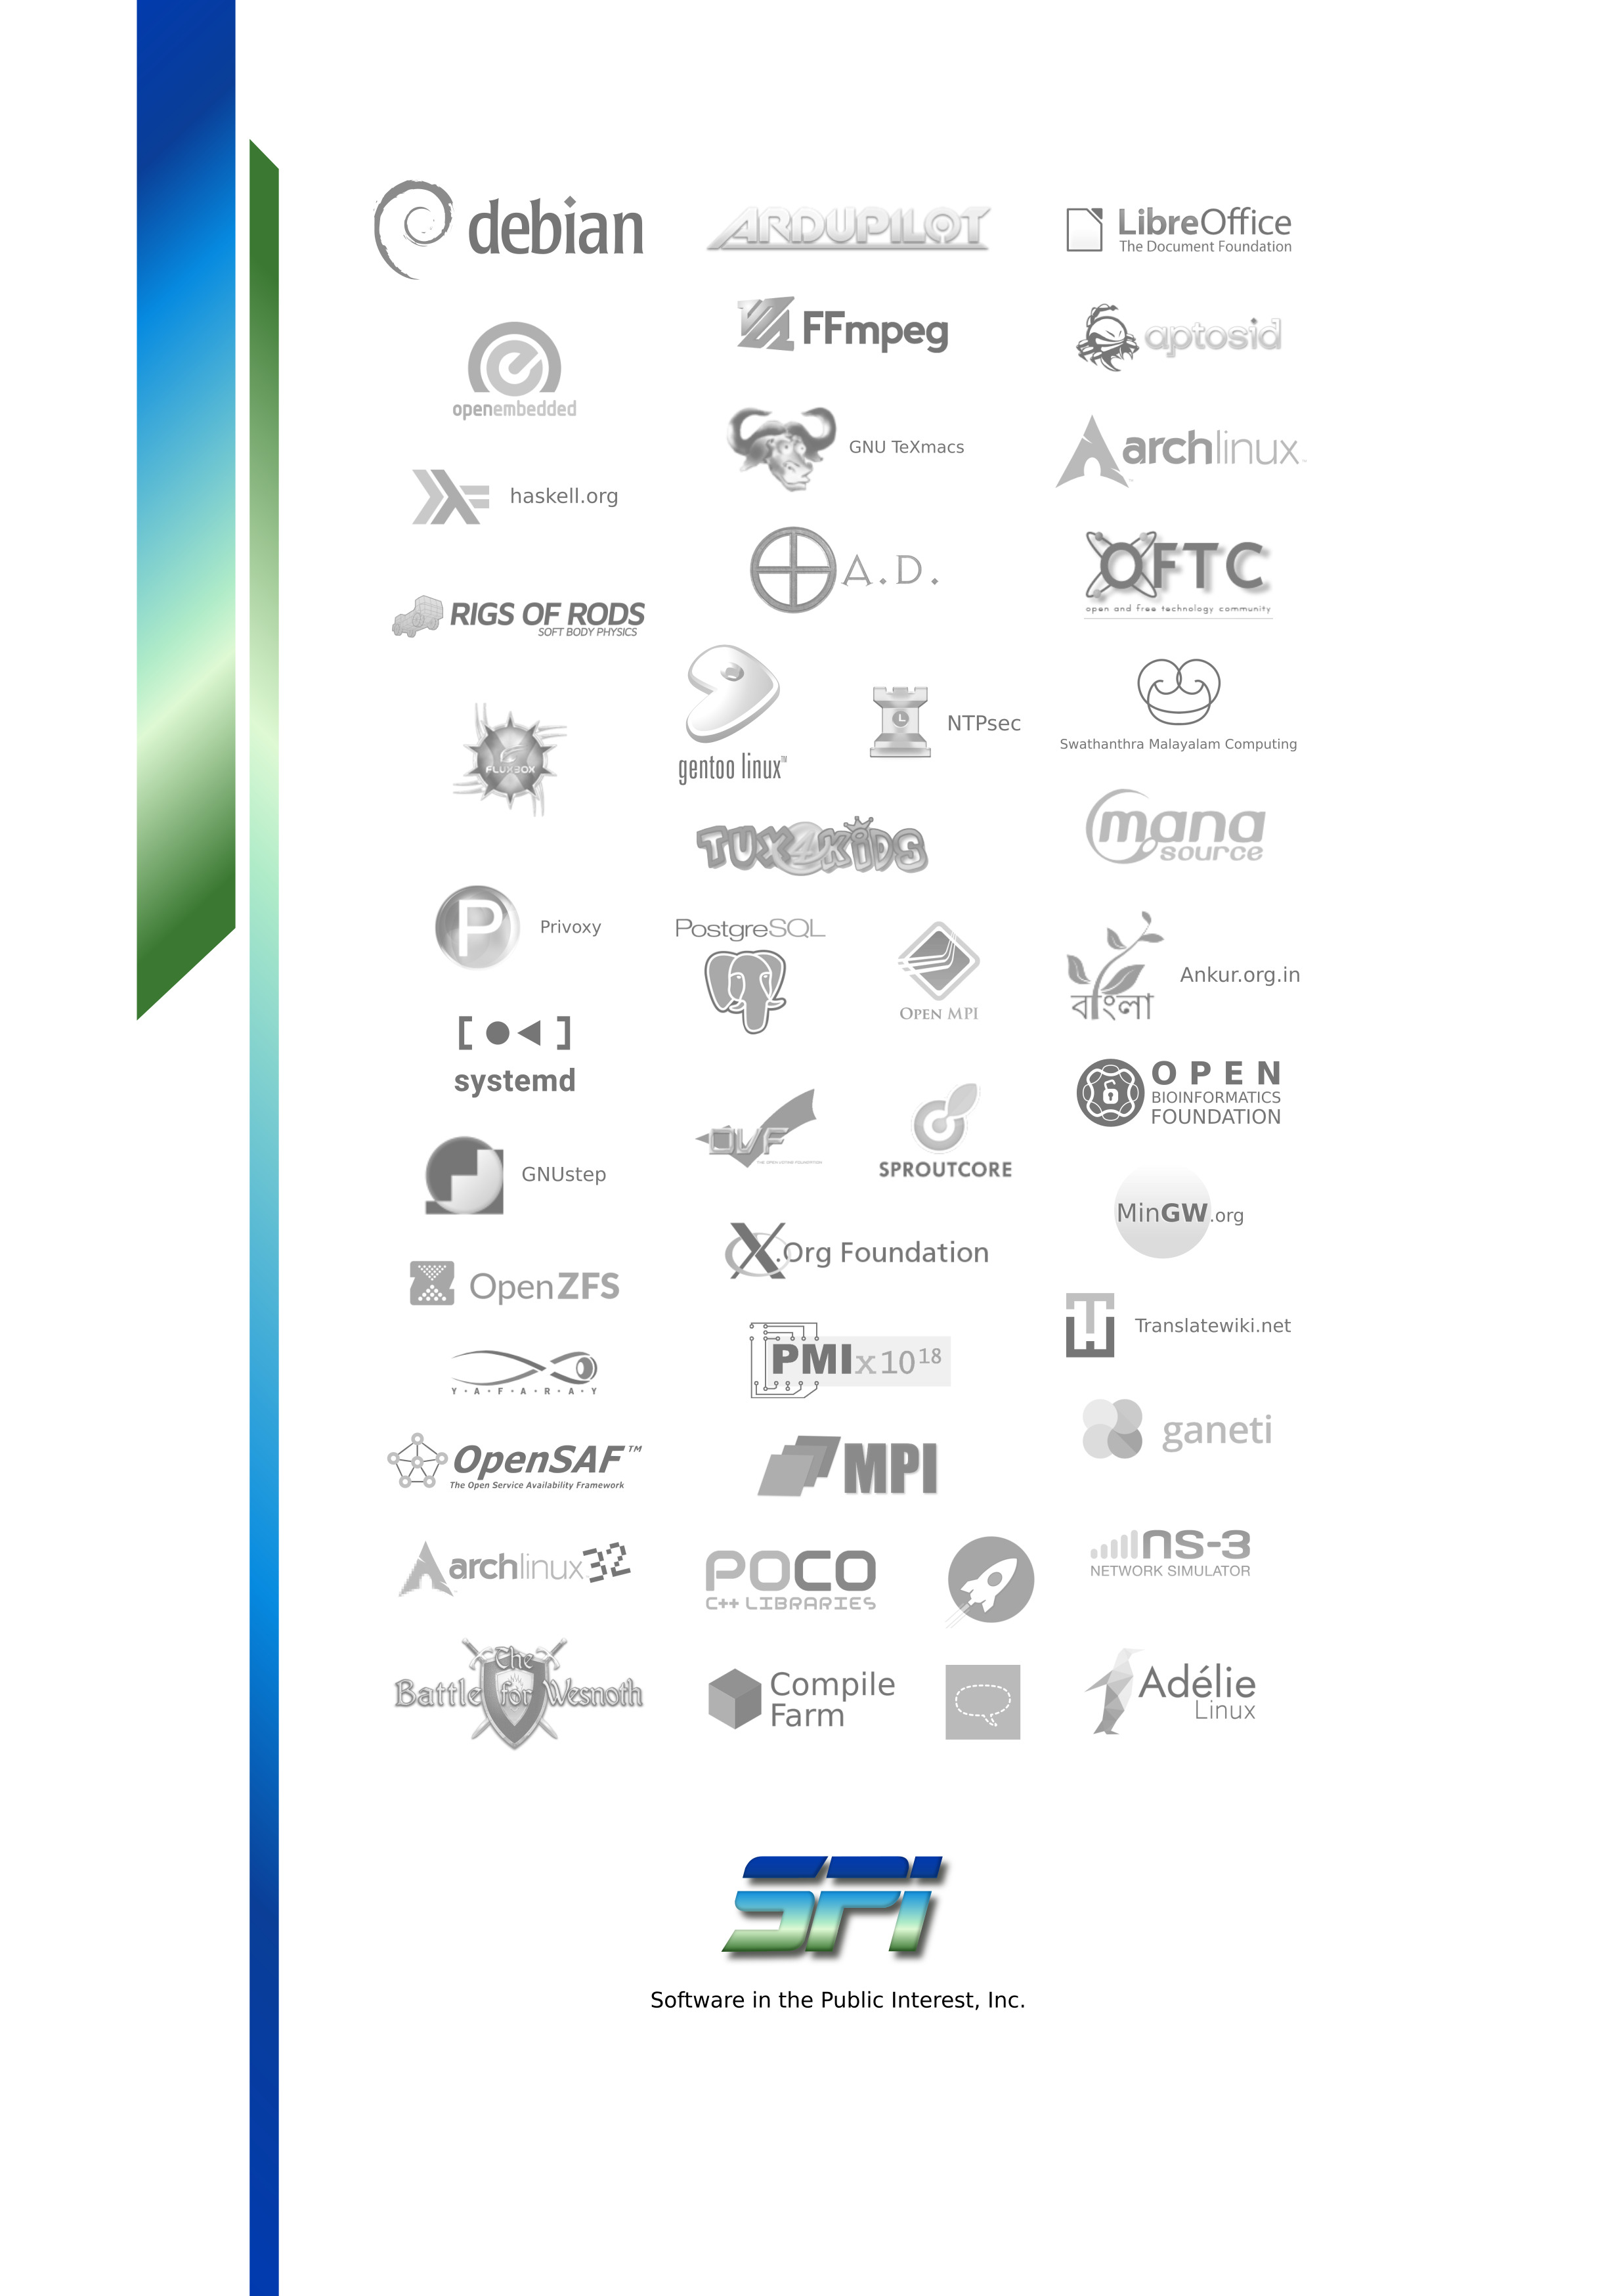
\includegraphics[width=\paperwidth,height=\paperheight]{images/spi-back-2024.jpg}}
}

\null

\end{document}
% Keep this at the bottom, thanks.
% Local Variables:
% TeX-master: "report"
% End:
